\documentclass[12pt,a4paper]{report}
\usepackage[english]{babel}
\usepackage{fontspec}
\setmainfont{Noto Serif}
\usepackage{geometry}
\geometry{
	top=25mm,
	bottom=25mm,
	left=30mm,
	right=25mm,
}
\usepackage{booktabs}
\usepackage{tikz}
\usetikzlibrary{calc}
\usetikzlibrary{matrix}
\usetikzlibrary{fit}
\usetikzlibrary{backgrounds}
\usetikzlibrary{decorations.pathmorphing}
\usetikzlibrary{arrows.meta, shapes.geometric, circuits.logic.US}
\usepackage{amsmath,amssymb}
\usepackage{graphicx}
\usetikzlibrary{shapes,arrows,positioning}
\usepackage{minted}
\usepackage{siunitx}
\sisetup{
	detect-all,
	range-phrase = {\,-\,},
	per-mode     = symbol,
	group-minimum-digits = 4
}
\usepackage[
colorlinks=true,
linkcolor=black,
urlcolor=blue,
citecolor=magenta
]{hyperref}
\usepackage{xcolor}

\newcommand{\hlref}[2]{%
	{\hypersetup{linkcolor=blue}%
		\hyperref[#1]{#2}}%
	\hypersetup{linkcolor=black}%
}

\hypersetup{
	pdftitle={Laomb: A Custom, Preemptive OS for a Legacy Pentium MMX System},
	pdfauthor={Jakub Lipový},
	pdfsubject={OS Design},
	pdfkeywords={Operating System, Assembly, Preemptive, Legacy Hardware, v8086, DOS},
}

\title{%
	Laomb: A Custom, Preemptive Operating System for a Legacy Pentium MMX Machine\\
	\large Leveraging Segmentation as Intel Intended
}
\author{Jakub Lipový\\
	NOVÝ PORG - Praha}
\date{\today}

\begin{document}
		
	\maketitle
		
	\begin{abstract}
	Laomb is a bespoke operating system targeting a single legacy desktop computer equipped with an Intel Pentium MMX (p5) processor.  
	Written in C and Assembly, and booted by a custom bootloader called Spark, it implements a fully preemptive kernel, including in-kernel preemption, using call-gate-based system calls and a ring-2 “driver” model to sandbox privileged extensions.  

	Both the kernel and userland employ a custom executable format, internally referred to as \texttt{binfmt}, which is detailed in section~\ref{sec:binfmt}. A key architectural decision is the first-class use of segmentation, not as a deprecated relic inferior to paging, but as a complementary mechanism for enforcing privilege and memory isolation.

	This paper presents the chronological development of Laomb: from hardware targeting and bootstrapping, through kernel core subsystems and userland execution, to modular driver infrastructure and a DOS compatibility layer.
	\end{abstract}
		
	\tableofcontents
	\listoffigures
	\listoftables

	\chapter{Motivation and Goals}

	The Laomb project began as a hands-on exploration of retrocomputing and low-level operating system design. After acquiring a vintage desktop PC equipped with a Pentium MMX processor, the opportunity arose to move beyond emulator-based experimentation and instead build a fully custom operating system, carefully tailored to run on real hardware.

	Having previously developed kernels targeting QEMU and modern x86 platforms, I sought to explore the peculiarities of 1990s-era PCs: constrained memory, legacy buses (ISA/PCI), BIOS interfaces, and the absence of modern standards such as ACPI or USB. Laomb emerged from this desire to build a minimal, performant, and precisely engineered OS for a single physical machine, exposing the full stack from firmware to userspace.

	\section{Rationale for Writing from Scratch}

	A defining decision in Laomb's development was to write nearly all components from scratch, rather than reuse or port existing tools. While this approach results in longer development time and potential initial inefficiencies, it provides complete control and visibility over each subsystem.

	Notable examples include:
	\begin{itemize}
		\item A custom bootloader (\texttt{spark}) in place of GRUB or Limine, to minimize dependencies and support early segmentation usage and custom executable format for the kernel.
		\item A custom executable format (\texttt{binfmt}) instead of ELF or PE, designed for simplicity, fast parsing and proper segmentation support.
		\item A non-POSIX userspace and syscall interface, discarding UNIX conventions in favor of a custom system with some familarities from NT or DOS, with segmentation-based memory protection and ring-2 drivers.
	\end{itemize}

	These decisions reflect an emphasis on experimental design and educational value, rather than compatibility or reusability.

	\section{Objectives and Scope}

	The primary goal of Laomb is to demonstrate a coherent and efficient OS architecture that:
	\begin{itemize}
		\item Exposes legacy PC subsystems and quirks through a clean and modular codebase.
		\item Validates a ring-2 driver sandboxing model using call gates for controlled privilege transitions.
		\item Restores segmentation as a practical tool for memory and privilege management, alongside paging.
	\end{itemize}

	\subsection{Design Constraints}

	The OS targets a fixed hardware configuration: a Pentium MMX-based desktop with 64~MiB of RAM, standard ISA and PCI devices, no ACPI, no USB, and basic BIOS functionality. As such, Laomb imposes the following limitations:

	\begin{itemize}
		\item \textbf{Hardware specialization:} The kernel assumes a single-core 32-bit CPU without SSE or 3DNow, and omits support for USB, ACPI, or hotplugging.
		\item \textbf{Software constraints:} All kernel and userspace code must fit within 64~MiB of RAM. Paging is enabled and used for memory protection; segmentation is relied upon heavily for NX regions.
		\item \textbf{Subsystem trade-offs:}
		\begin{itemize}
			\item \textbf{Networking:} Only legacy 10 Mbps Ethernet via NE2000-compatible PCI NICs, with support for static IP, UDP, and TCP.
			\item \textbf{Graphics:} Basic framebuffer graphics using Cirrus Logic PCI VGA cards, with no acceleration or high-resolution modes.
		\end{itemize}
	\end{itemize}

	These constraints promote determinism, simplify debugging, and enforce tight coupling between software and hardware.

	
	\chapter{Target Hardware}
	\label{chap:target-hardware}
	
	\section{System Specifications}
	
	The target system for \emph{Laomb} is a single Pentium MMX-class desktop PC with \SI{64}{\mebi\byte} of RAM and a mixture of legacy ISA and PCI devices. A detailed overview of each major hardware component is provided, including processor features, memory organization, I/O peripherals, and chipset architecture.
	
	\subsection{CPU: Intel Pentium MMX (i586)}
	\label{sec:cpu}
	
	The central processing unit is an Intel Pentium MMX (i586) running at approximately \SI{166.1}{\mega\hertz}. The MMX extension adds a set of 57 new SIMD instructions and \SI{64}{\bit} of additional register state (the MMX registers alias the x87 floating-point registers). Key technical details are as follows:
	
	\begin{itemize}
		\item \textbf{Model:} Intel Pentium MMX (p5 microarchitecture, i586 compiler target)
		\item \textbf{Clock Speed:} \SI{166.1}{\mega\hertz} (nominal)
		\item \textbf{L1 Cache:} 
		\begin{itemize}
			\item \SI{16}{\kibi\byte} Instruction cache
			\item \SI{16}{\kibi\byte} Data cache
		\end{itemize}
		\item \textbf{L2 Cache:} \SI{512}{\kibi\byte} Synchronous Pipelined Burst SRAM (on-die, write-back)
		\item \textbf{Math Co-Processor:} Integrated x87 FPU with MMX register aliasing
		\item \textbf{Bus Interface:} 
		\begin{itemize}
			\item PCI v2.10 (\SI{33}{\mega\hertz}, 32-bit data path)
			\item ISA (8-bit/16-bit legacy bus, \SI{8}{\mega\hertz})
		\end{itemize}
	\end{itemize}
	
	Since Laomb targets a single fixed CPU model, the kernel's assembly stubs were optimized for the Pentium MMX's microarchitecture, taking advantage of pipelined integer units and the on-die L2 cache. The integrated FPU/MMX unit simplifies floating-point or multimedia workloads, if any, inside userspace, as the kernel correctly handles lazy loading of a user thread's ability to use them.
	
	\subsection{Memory: \SI{64}{\mebi\byte} DRAM}
	\label{sec:memory}
	
	The system has a total of \SI{64}{\mebi\byte} of DRAM, organized as four banks of synchronous DRAM chips.
	
	\noindent\textbf{DRAM Configuration:}
	\begin{itemize}
		\item Banks 0/1 and 2/3 populated with synchronous DRAM modules
		\item All chips operate in burst-access mode at system clock
		\item No parity or ECC
	\end{itemize}
	
	To visualize the physical memory layout, see Figure~\ref{fig:memory-map}.
	
	\begin{figure}[ht]
		\centering
		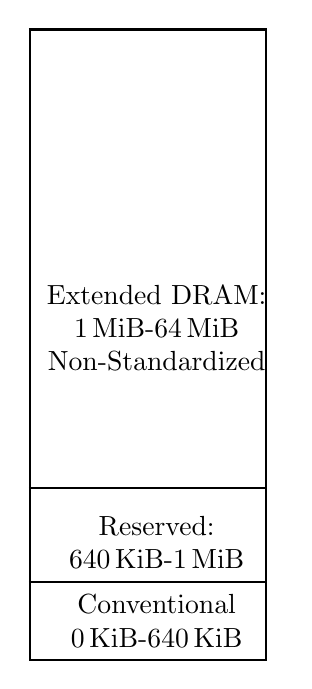
\begin{tikzpicture}[
			memory/.style = {draw, thick, minimum width=3cm, inner sep=2pt},
			region/.style = {minimum height=1cm, draw=none, text width=3cm, align=center}
			]
			\coordinate (base) at (0,0);
			\node[memory, minimum height=8cm, anchor=south west] (mem) at (base) {};
			
			\node[region, anchor=south west] at (mem.south west) (conv) {Conventional\\\SI{0}{\kibi\byte}-\SI{640}{\kibi\byte}};
			\draw[thick] ($(mem.south west) + (0,1cm)$) -- ($(mem.south west) + (3cm,1cm)$);
			
			\node[region, anchor=south west] at ($(mem.south west)+(0,1cm)$) (res) {Reserved:\\\SI{640}{\kibi\byte}-\SI{1}{\mebi\byte}};
			\draw[thick] ($(mem.south west) + (0,2.2cm)$) -- ($(mem.south west) + (3cm,2.2cm)$);
			
			\node[region, anchor=south west] at ($(mem.south west)+(0,3.5625cm)$) (ext) {Extended DRAM:\\\SI{1}{\mebi\byte}-\SI{64}{\mebi\byte}\\Non-Standardized};
			\draw[thick] ($(mem.north west)$) -- ($(mem.north east)$);
		\end{tikzpicture}
		\caption{Physical Memory Layout of the Pentium MMX System.}
		\label{fig:memory-map}
	\end{figure}
	
	In Laomb, the first \SI{1}{\mebi\byte} is reserved for real-mode boot and BIOS data structures. The extended region (\SI{1}{\mebi\byte}-\SI{64}{\mebi\byte}) is managed by a bitmap-based frame allocator. Shadow/Special RAM (\SI{384}{\kibi\byte}) is used for BIOS shadowing to improve fetch performance at boot.
	
	\subsection{Input Devices: 5-pin DIN Keyboard, PS/2 Mouse; Serial/Parallel Ports}
	\label{sec:input}
	
	The input subsystem comprises legacy PS/2 connectors and standard ISA serial/parallel ports. Details:
	
	\begin{itemize}
		\item \textbf{Keyboard Controller:} 5-pin DIN keyboard uses an i8042-compatible controller.
		\item \textbf{Super I/O Chip:} Winbond W83877F - provides PS/2 keyboard/mouse interfaces, two UARTs, one parallel port, and floppy controller registers.
		\item \textbf{Serial Ports:}
		\begin{itemize}
			\item \textbf{COM1:} 16550A UART, I/O base \texttt{0x3F8}, IRQ 4, FIFO enabled
			\item \textbf{COM2:} 16550A UART, I/O base \texttt{0x2F8}, IRQ 3, FIFO enabled
		\end{itemize}
		\item \textbf{Parallel Port:}
		\begin{itemize}
			\item \textbf{LPT1:} 4-bit Standard Parallel Port (SPP), I/O base \texttt{0x378}, IRQ 7
			\item \textbf{LPT2/3:} Not present
		\end{itemize}
		\item \textbf{Floppy Disk Controller (FDC):} Integrated in W83877F, uses standard I/O registers at \texttt{0x3F0}-\texttt{0x3F7} and IRQ 6. Supports 3.5'' \SI{1.44}{\mega\byte} drives.
	\end{itemize}
	
	An early debug console utilized the 16550A UART at COM1 (\texttt{0x3F8}, IRQ 4) for reliable serial output. PS/2 keyboard scancodes are handled via the i8042 controller's ports \texttt{0x60}/\texttt{0x64}, enabling input in both kernel and userspace.
	
	\subsection{Graphics and Sound}
	\label{sec:video-audio}
	
	A PCI-bus VGA adapter is combined with an ISA-bus audio card. Both subsystems are essential for user interaction and debugging on real hardware.
	
	\subsubsection{Graphics: Cirrus Logic CL-GD5436 (PCI)}
	\begin{itemize}
		\item \textbf{Chipset:} Cirrus Logic CL-GD5436, codename \emph{Alpine}.
		\item \textbf{VRAM:} \SI{2}{\mebi\byte} DRAM (\SI{256}{\kibi\byte} × 8 banks).
		\item \textbf{RAMDAC:} Cirrus Internal CL24 TrueColor (supports 24-bit color).
		\item \textbf{Video BIOS:} Version 1.00, mapped at segment \texttt{0xC000} (\SI{32}{\kibi\byte}).
		\item \textbf{Bus:} PCI (function 0, video class) - supports VESA VBE 1.2.
		\item \textbf{Modes:} VGA \num{640}×\num{480}×\num{16}\,colors; Super VGA up to \num{800}×\num{600}×\num{256}\,colors; VESA text modes via BIOS.
	\end{itemize}
	
	Usage in Laomb: A minimal SVGA driver is loaded via VESA BIOS Extensions (VBE 1.2) during early boot. For advanced text console or graphical framebuffer operations, the PCI BAR corresponding to the VRAM region \texttt{0xA0000-0xBFFFF} is mapped into higher-half kernel space.
	
	\subsubsection{Audio: C-Media CMI8330 ISA Adapter (Sound Blaster Pro Compatible)}
	\begin{itemize}
		\item \textbf{Chipset:} CMI8330, ISA-bus, Sound Blaster Pro 2.0-compatible.
		\item \textbf{I/O Ports:} \texttt{0x220-0x22F}.
		\item \textbf{DMA Channels:} 1 (8-bit DMA), 5 (16-bit DMA).
		\item \textbf{IRQ:} 11.
		\item \textbf{Features:} \SI{8}{\bit} and \SI{16}{\bit} PCM audio; joystick/MIDI via MPU-401 interface.
	\end{itemize}
	
	Usage in Laomb: A minimal SB Pro driver is implemented to program DMA transfers for simple beep or waveform data, primarily to validate low-level DMA handling in ring-2 driver mode. Full MPU-401 emulation is deferred to the DLCL when running legacy DOS games.
	
	\subsection{Network: Realtek RTL8029(AS) Ethernet (PCI)}
	\label{sec:network}
	
	The network interface is a Realtek RTL8029(AS), which is NE2000-compatible over PCI. Key details:
	
	\begin{itemize}
		\item \textbf{Chipset:} RTL8029(AS) (PCI device ID 10EC:8029).
		\item \textbf{I/O Ports:} Determined by PCI BAR (standard NE2000 register offsets).
		\item \textbf{IRQ:} 10.
		\item \textbf{DMA:} Supports 16-bit bus-master DMA for packet transfers.
		\item \textbf{Features:} 10 Mbps Ethernet, full/half-duplex via auto-negotiation, on-chip FIFO and MAC.
	\end{itemize}
	
	Usage in Laomb: A lightweight NE2000 driver is built in ring-2, using the PCI bus master registers to enqueue and dequeue packet buffers. The RTL8029's NE2000 compatibility allows reuse of well-known driver logic from OSDev resources.
	
	\subsection{Storage and I/O Controllers}
	\label{sec:storage-io}
	
	Storage is provided by an IDE hard disk, an ATAPI CD-ROM, and a floppy drive controller. The controllers and their capabilities are detailed below.
	
	\subsubsection{IDE Hard Disk (VIA VT82C571)}
	\begin{itemize}
		\item \textbf{Controller:} VIA VT82C571 (integrated IDE on Apollo VP-1 chipset).
		\item \textbf{Disk Model:} M61641TA.
		\item \textbf{Capacity:} \SI{1040}{\mebi\byte} (1 091 026 944 bytes).
		\item \textbf{Geometry:} 2 114 cylinders, 16 heads, 63 sectors/track.
		\item \textbf{Cache Buffer:} \SI{64}{\kibi\byte}.
		\item \textbf{PIO Mode:} 4 (maximum PIO transfer rate \SI{16.6}{\mebi\byte\per\second}).
		\item \textbf{DMA Modes:} SWDMA 2 (\SI{16.7}{\mebi\byte\per\second}), MWDMA 2 (\SI{33.3}{\mebi\byte\per\second}).
		\item \textbf{Features:} Multiple Sector Buffer, Read Cache, LBA, IORDY.
	\end{itemize}
	
	The IDE driver initializes the controller in UDMA-disabled mode (simpler timing) and uses the 32-bit PIO interface for early testing. Later, MWDMA 2 is enabled for improved throughput. Both CHS and LBA addressing are supported.
	
	\subsubsection{ATAPI CD-ROM (VIA VT82C571)}
	\begin{itemize}
		\item \textbf{Controller:} Same VIA VT82C571 IDE interface.
		\item \textbf{Drive Model:} ATAPI CDROM 2.30TW240D.
		\item \textbf{Max Speed:} 24× (\SI{4253}{\kibi\byte\per\second}).
		\item \textbf{Buffer:} \SI{120}{\kibi\byte}.
		\item \textbf{PIO Mode:} 4.
		\item \textbf{DMA Mode:} SWDMA 2, MWDMA 1.
		\item \textbf{Features:} LBA, DMA, IORDY, Audio Play, Photo CD, Multisession.
	\end{itemize}
	
	In Laomb, PACKET commands (\texttt{0xA0}) are issued over the IDE command block. LBA and PIO modes are verified, with a fallback to SWDMA if timing issues arise on real hardware. A basic CDROM filesystem driver (ISO 9660) is layered on top.
	
	\subsubsection{Floppy Disk Controller (FDC)}
	\begin{itemize}
		\item \textbf{Chipset:} Integrated in Winbond W83877F Super I/O.
		\item \textbf{Drive Type:} 3.5'' \SI{1.44}{\mega\byte} (2 head, 80 track, 18 sectors/track).
		\item \textbf{I/O Ports:} \texttt{0x3F0-0x3F7}.
		\item \textbf{IRQ:} 6.
		\item \textbf{DMA:} Channel 2 (for floppy DMA transfers).
	\end{itemize}
	
	The floppy driver programs the standard Intel 82077AA command set for seek, read, write, and recalibrate. DMA channel 2 is used to transfer \SI{512}{\byte} per sector at \SI{300}{\kibi\byte\per\second}.
	
	\subsection{Southbridge \& Chipset Architecture}
	\label{sec:southbridge}
	
	The motherboard is a FIC PA-2006 series, built around the VIA Apollo VP-1 chipset (VT82C580VP northbridge + VT82C571 southbridge). The Award Modular BIOS v4.51PG (dated 04/08/1997) configures the following:
	
	\begin{itemize}
		\item \textbf{Northbridge (VT82C580VP):}
		\begin{itemize}
			\item Connects CPU to PCI bus and DRAM.
			\item Provides AGP/PCI arbiter and memory controller.
		\end{itemize}
		\item \textbf{Southbridge (VT82C571):}
		\begin{itemize}
			\item Integrated IDE (two channels: Primary/Secondary).
			\item ISA bridge, super I/O (floppy, serial, parallel).
			\item Real Time Clock (RTC) and CMOS.
			\item Programmable Interrupt Controller (PIC) cascaded to master/slave.
			\item DMA controller (channels 0-7).
		\end{itemize}
		\item \textbf{Award BIOS Features:}
		\begin{itemize}
			\item \emph{BIOS32 Services:} Present (enables 32-bit protected-mode entry).
			\item \emph{Plug-and-Play:} Present (v1.0).
			\item \emph{APM:} Present (v1.2).
			\item \emph{ACPI:} Not present.
		\end{itemize}
	\end{itemize}
	
	\begin{figure}[ht]
		\centering
		\resizebox{\textwidth}{!}{%
			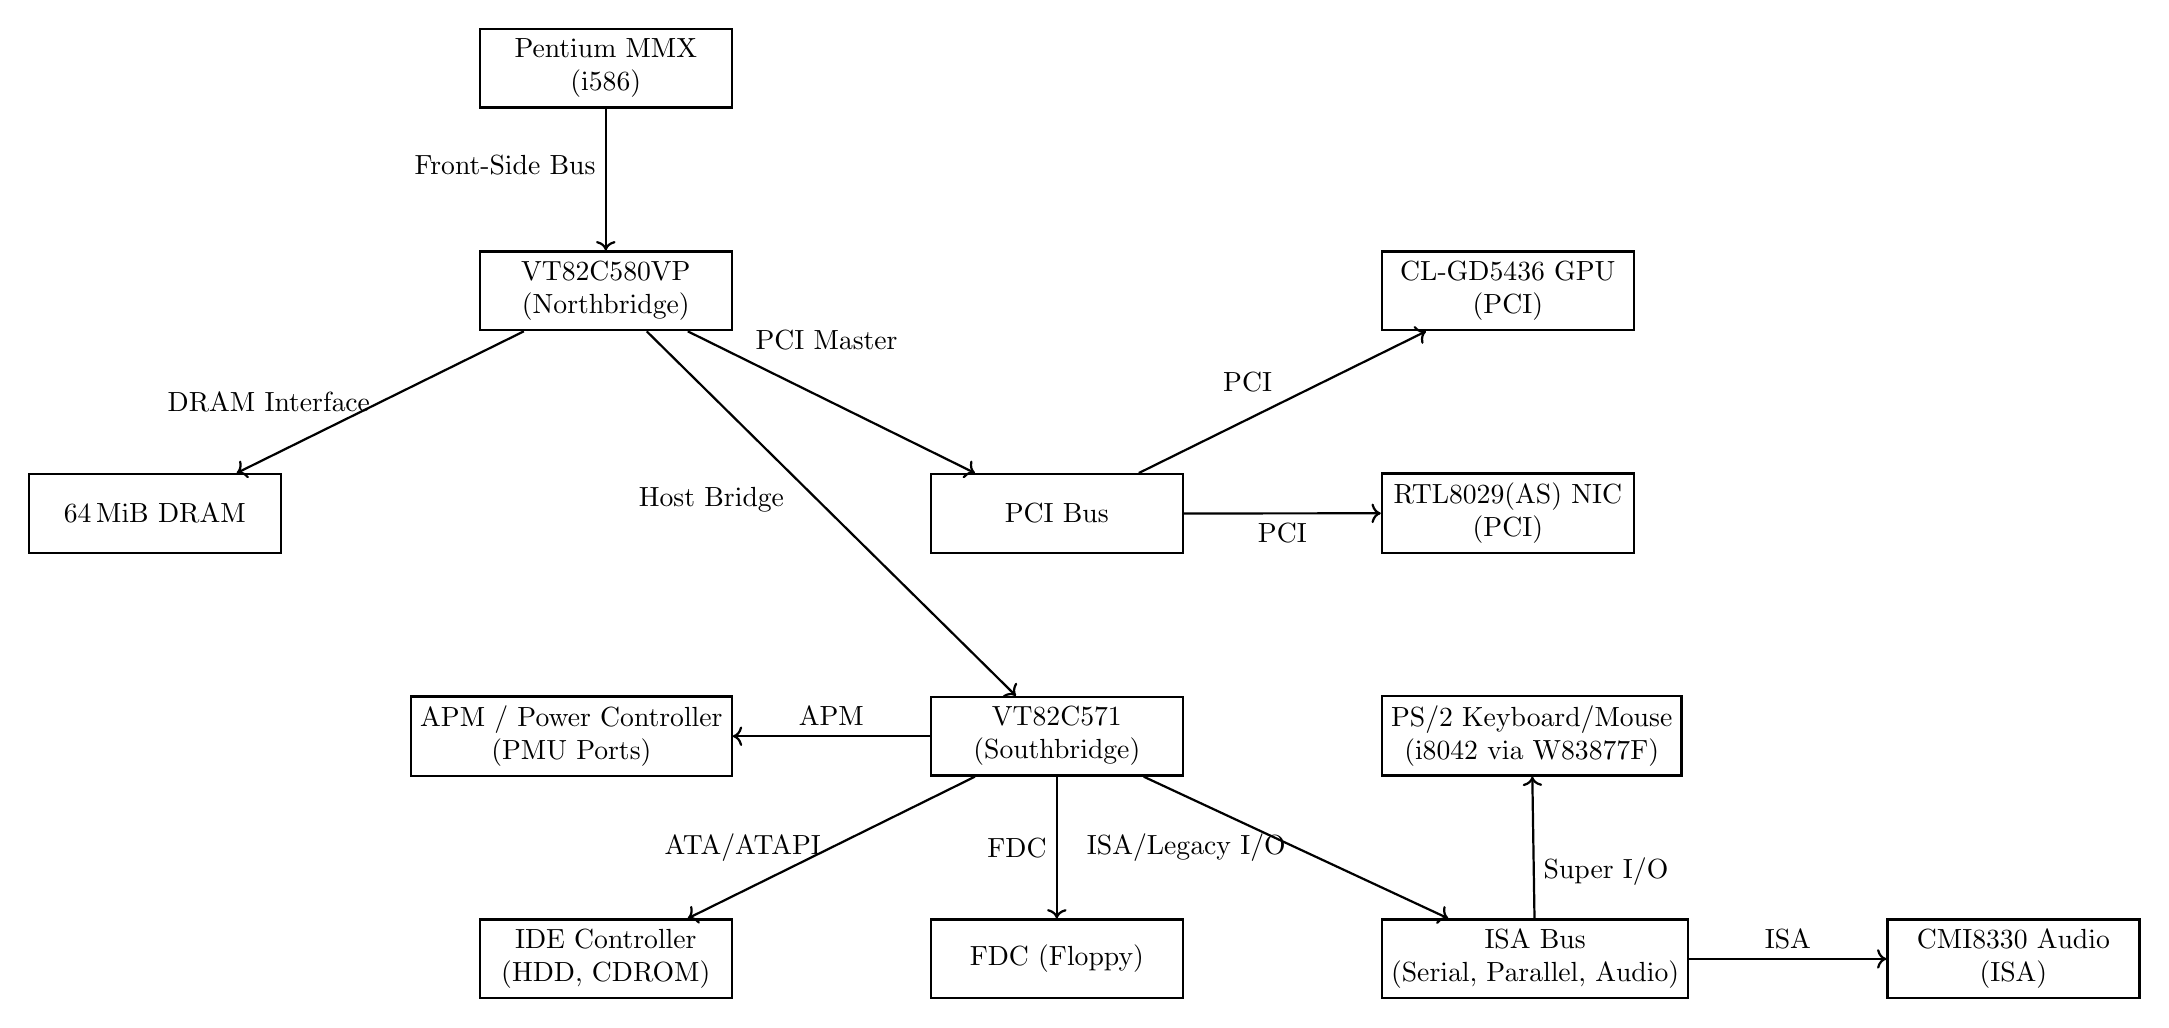
\begin{tikzpicture}[
				node distance=1.8cm and 2.5cm,
				box/.style = {draw, thick, minimum width=3.2cm, minimum height=1cm, align=center},
				line/.style = {->, thick}
				]
				
				\node[box] (cpu) {Pentium MMX\\(i586)};
				\node[box, below=of cpu] (north) {VT82C580VP\\(Northbridge)};
				\node[box, below left=of north] (dram) {\SI{64}{\mebi\byte} DRAM};
				\node[box, below right=of north] (pci) {PCI Bus};
				\node[box, above right=of pci] (gpu) {CL-GD5436 GPU\\(PCI)};
				\node[box, below=of pci] (south) {VT82C571\\(Southbridge)};
				\node[box, left=of south] (apm) {APM / Power Controller\\(PMU Ports)};
				\node[box, below left=of south] (ide) {IDE Controller\\(HDD, CDROM)};
				\node[box, below=of south] (fib) {FDC (Floppy)};
				\node[box, below right=of south] (io) {ISA Bus\\(Serial, Parallel, Audio)};
				\node[box, right=of io] (audio) {CMI8330 Audio\\(ISA)};
				\node[box, above right=of fib] (kbm) {PS/2 Keyboard/Mouse\\(i8042 via W83877F)};
				\node[box, above right=of south] (rtl) {RTL8029(AS) NIC\\(PCI)};
				
				\draw[line] (cpu) -- (north) node[pos=0.4,left] {Front-Side Bus};
				\draw[line] (north) -- (dram) node[midway,left] {DRAM Interface};
				\draw[line] (north) -- (pci) node[pos=0.2,above right] {PCI Master};
				\draw[line] (pci) -- (gpu) node[midway,above left] {PCI};
				\draw[line] (pci) -- (rtl) node[midway,below] {PCI};
				\draw[line] (north) -- (south) node[pos=0.4,below left] {Host Bridge};
				\draw[line] (south) -- (ide) node[midway,left] {ATA/ATAPI};
				\draw[line] (south) -- (fib) node[midway,left] {FDC};
				\draw[line] (south) -- (io) node[midway,left] {ISA/Legacy I/O};
				\draw[line] (south) -- (apm) node[midway,above] {APM};
				\draw[line] (io) -- (audio) node[midway,above] {ISA};
				\draw[line] (io) -- (kbm) node[midway,below right] {Super I/O};
			\end{tikzpicture}
		}
		\caption{Simplified Block Diagram of VIA Apollo VP-1 Chipset and Peripheral Interconnects.}
		\label{fig:chipset-block}
	\end{figure}
	
	\subsection{IRQ Routing and DMA Channels}
	\label{sec:irq-routing}
	
	The Award BIOS configures IRQs and DMA channels as shown in Table~\ref{tab:irq-mapping}. Laomb's interrupt manager programs the 8259A PIC cascade in accordance with this mapping.
	
	\begin{table}[ht]
		\centering
		\begin{tabular}{c p{8cm}}
			\toprule
			\textbf{IRQ} & \textbf{Device} \\
			\midrule
			0   & System Timer (8253/8254 PIT) \\
			1   & Keyboard Controller (i8042) \\
			2   & Cascade Output from Slave PIC \\
			3   & COM2 (Serial Port, \texttt{0x2F8}) \\
			4   & COM1 (Serial Port, \texttt{0x3F8}) \\
			5   & Free / LPT2 (Parallel Port 2) \\
			6   & Floppy Disk Controller (FDC) \\
			7   & Parallel Port LPT1 (\texttt{0x378}) \\
			8   & Real-Time Clock (RTC) \\
			9   & IRQ2 Rerouted (usually unused) \\
			10  & RTL8029(AS) Ethernet (PCI) \\
			11  & CMI8330 Audio (ISA) \\
			12  & Free / PS/2 Mouse (via i8042) \\
			13  & Numeric Data Processor (x87 FPU/MMX exception) \\
			14  & Primary IDE Channel (HDD) \\
			\bottomrule
		\end{tabular}
		\caption{IRQ Assignments on the Pentium MMX System.}
		\label{tab:irq-mapping}
	\end{table}
	
	Similarly, DMA channels are allocated as follows (managed by the VT82C571 southbridge's integrated DMA controller):
	
	\begin{itemize}
		\item \textbf{DMA 0/1/3/5/6/7:} Available for general use (not reserved).
		\item \textbf{DMA 2:} Floppy Disk Controller (FDC).
		\item \textbf{DMA 1:} ISA Audio (CMI8330) for 16-bit transfers.
		\item \textbf{DMA 5:} ISA Audio (CMI8330) for 8-bit transfers.
		\item \textbf{DMA 4:} Cascade for second DMA controller (channels 4-7).
	\end{itemize}
	
	In Laomb, these channels are assumed to be non-volatile. The data transfers are sequenced for ATA and audio devices.
	
	\chapter{Spark Bootloader}
	\section{Boot Process}

	% TODO subsections...
	
	\section{Loader Handoff and Memory Map Parsing}

	% TODO
	
	\chapter{Binfmt Executable Format}
	\label{sec:binfmt}
	\section{Core Executable Format Design}

	\section{Executable Format Specification}
	
	\section{Linux Userspace Linker Implementation}

	\section{Spark Dynamic Linker}

	\chapter{Global Descriptor Table and Call Gates}
	\section{GDT Setup}
	
	\section{Call Gate Stubs and Future Syscall Planning}

	\chapter{Interrupt Descriptor Table and IRQ Handling}
	\section{IDT Initialization}
	
	\section{Exception and Interrupt Handlers}
	
	\chapter{Programmable Interrupt Controller and Timer}
	\section{PIC (8259) Configuration}
	
	\section{PIT (8254) Setup}
	
	\chapter{Physical Memory Management}
	\section{Parsing the BIOS-Provided Memory Map}
	
	\section{Bitmap-Based Frame Allocator}
	
	\chapter{Virtual Memory and Kernel Heap}
	\section{x86 Paging Structures}
	
	\section{Paging Manager Implementation}
	
	\section{Kernel Heap (SLUB) Allocator}
	
	\chapter{Process Scheduler}
	\section{Task Structure and Context Switching}
	
	\section{Scheduling Algorithm and Preemption}
	
	\chapter{Virtual File System}
	\section{VFS Abstractions}
	
	\section{File and Directory Interfaces}
	
	\chapter{Filesystems}
	\section{Master Boot Record and Partition Tables}
	
	\section{RealFS: FAT32 Implementation}
	
	\chapter{Userland Loading}
	\section{Kernel ELF Loader}
	
	\section{Kernel Dynamic Linker}
	
	\section{Ring-3 Transition Mechanism}
	
	\chapter{System Call Implementation}
	\section{Call Gate Mechanism}
	
	\section{Syscall ABI and Dispatch Logic}
	
	\chapter{Device Drivers}
	\section{Floppy Disk Controller (FDC)}
	
	\section{ATAPI CD-ROM Driver}

	\section{RTL8029AS Network Card}
	
	\section{C-Media CMI8330 (Sound Blaster Pro compatible) Driver}
	
	\section{Cirrus Logic GD-5446 GPU}
	
	\chapter{Southbridge and Power Management}
	\section{Reversing APM BIOS}
	
	\section{Direct Southbridge Interaction}
	
	\chapter{Userspace Environment}
	\section{Custom \texttt{libc}}
	
	\section{Init System and Shell}
	
	\section{Userland Task Management}
	
	\chapter{Real Hardware Bring-Up}
	\section{Booting on the Target Device}
	
	\section{Debugging and Validation Challenges}
	
	\chapter{Ring-2 Driver Model}
	\section{Driver Process Architecture}
	
	\section{I/O and MMIO Access Control}
	
	\section{Kernel Callback Registration}
	
	\chapter{DOS Laomb Compatibility Layer (DLCL)}
	\section{Simple v8086 Driver Prototype}

	\section{Full DOS Emulation Integration}
	
	\section{Integration with VFS, Networking, and Drivers}
	
	\chapter{Conclusion}
	\section{Summary of Development Journey}
	
	\section{Lessons Learned}

	\section{Future Work}

	\cleardoublepage
	\begin{thebibliography}{99}
		\addcontentsline{toc}{chapter}{Bibliography}
		
		\bibitem{intel_sdm}
		Intel Corporation.  
		\textit{Intel 64 and IA-32 Architectures Software Developer's Manual, Vols. 1-3}.  
		2023.  
		\url{https://www.intel.com/content/www/us/en/developer/articles/technical/intel-sdm.html}
		
		\bibitem{intel_pentium_mmx_sdm}
		Intel Corporation.  
		\textit{Pentium Processor Family Developer's Manual: Volume 3-Architecture and Programming}.  
		1996.  
		\url{ftp://download.intel.com/design/pentium/manuals/24142805.pdf}
		
		\bibitem{apm12}
		Compaq, IBM, Phoenix Consortium \& Microsoft.  
		\textit{Advanced Power Management (APM) BIOS Interface Specification, Version 1.2}.  
		1996.  
		\url{https://stuff.mit.edu/afs/sipb/contrib/doc/specs/protocol/apm12.pdf}
		
		\bibitem{cmedia_cmi8330}
		C-Media Electronics, Inc.  
		\textit{CMI8330A/C3D Plug-and-Play Audio Chip Datasheet}.  
		Accessed May 30, 2025.  
		\url{https://dosdays.co.uk/media/cmedia/CMI8330_Datasheet.pdf}
		
		\bibitem{sbpro}
		Creative Technology.  
		\textit{Sound Blaster Pro User Reference Manual}.  
		1992.  
		\url{https://www.manualslib.com/manual/3586527/Creative-Sound-Blaster-Pro.html}
		
		\bibitem{rtl8029as}
		Realtek Semiconductor Corp.  
		\textit{RTL8029AS PCI Full-Duplex Ethernet Controller Advanced Information}.  
		1997.  
		\url{https://realtek.info/pdf/rtl8029as.pdf}
		
		\bibitem{ne2000}
		Novell Ltd.  
		\textit{Operations Manual LPM/MCM-NE2000}.  
		1995.  
		\url{https://resources.winsystems.com/product-manuals/lpmmcm-ne2000-pm.pdf}
		
		\bibitem{cirrus_gd5446}
		Cirrus Logic, Inc.  
		\textit{CL-GD5446 Preliminary Data Book}.  
		1996.  
		\url{https://www.alldatasheet.com/datasheet-pdf/pdf/78538/CIRRUS/CL-GD5446.html}
		
		\bibitem{rcollins_f00b_bug}
		R. Collins.  
		“Pentium ‘F00F' Erratum: The Pentium F00F Bug.”  
		Dec. 1997.  
		\url{https://www.rcollins.org/Errata/Dec97/F00FBug.html}
		
		\bibitem{kleiman_vnodes}
		S. R. Kleiman.  
		“Vnodes: An Architecture for Multiple File System Types in Sun UNIX.”  
		\textit{Software-Practice \& Experience}, 17(7):727-761, Jul. 1987.  
		\url{https://www.cs.fsu.edu/~awang/courses/cop5611_s2024/vnode.pdf}
		
		\bibitem{osdev_mbr}
		OSDev Wiki.  
		“Master Boot Record (x86).”  
		Accessed May 30, 2025.  
		\url{https://wiki.osdev.org/MBR_(x86)}
		
		\bibitem{osdev_fat32}
		OSDev Wiki.  
		“FAT32.”  
		Accessed May 30, 2025.  
		\url{https://wiki.osdev.org/FAT32}
		
		\bibitem{wiki_fat32}
		Wikipedia.  
		“FAT32.”  
		Accessed May 30, 2025.  
		\url{https://en.wikipedia.org/wiki/FAT32}
		
		\bibitem{8259}
		Intel Corporation.  
		\textit{8259A Programmable Interrupt Controller Data Sheet}.  
		1988.  
		\url{https://pdos.csail.mit.edu/6.828/2010/readings/hardware/8259A.pdf}
		
		\bibitem{8254}
		Intel Corporation.  
		\textit{8254 Programmable Interval Timer Data Sheet}.  
		1993.  
		\url{https://www.scs.stanford.edu/10wi-cs140/pintos/specs/8254.pdf}
		
		\bibitem{fdc_spec}
		IBM.  
		\textit{82077AA CHMOS Single-Chip Floppy Disk Controller Data Sheet}.  
		1987.  
		\url{http://www.osdever.net/documents/82077AA_FloppyControllerDatasheet.pdf?the_id=41}
		
		\bibitem{brokenthorn_pm}
		Brokenthorn Entertainment.  
		“Protected Mode Basics Part 1.”  
		\textit{Brokenthorn OS Development Series}, 2009.  
		\url{http://www.brokenthorn.com/Resources/OSDev20.html}
		
		\bibitem{atapi_ata}
		INCITS (ANSI).  
		\textit{ATA/ATAPI Command Set (ANSI INCITS 515-2012)}.  
		2013.  
		\url{https://read.seas.harvard.edu/cs161/2019/pdf/ata-atapi-8.pdf}
		
		\bibitem{hyper_loader}
		Hyper OS Project.  
		“Hyper Bootloader.”  
		Accessed May 30, 2025.  
		\url{https://github.com/UltraOS/Hyper}
		
		\bibitem{lwn_slub229984}
		A. Dunham.  
		“The SLUB Allocator.”  
		LWN.net, Apr. 2007.  
		\url{https://lwn.net/Articles/229984/}
		
		\bibitem{ms_peb}
		Microsoft Docs.  
		“PEB (Process Environment Block) Structure (winternl.h).”  
		Accessed May 30, 2025.  
		\url{https://learn.microsoft.com/en-us/windows/win32/api/winternl/ns-winternl-peb}
		
		\bibitem{elf_spec}
		T. Lindholm et al.  
		\textit{Executable and Linking Format (ELF) Specification}.  
		Linux Foundation, 2015.  
		\url{https://refspecs.linuxfoundation.org/elf/elf.pdf}
		
		\bibitem{ralfbrown}
		Ralf Brown.  
		“Interrupt List.”  
		Carnegie Mellon University. Accessed May 30, 2025.  
		\url{https://www.cs.cmu.edu/~ralf/files.html}
		
		\bibitem{ibm_bios}
		IBM.  
		\textit{PS/2 and PC BIOS Interface Technical Reference}.  
		Apr. 1987.  
		\url{https://web.archive.org/web/20180514201215/https://classiccomputers.info/down/IBM_PS2/documents/PS2_and_PC_BIOS_Interface_Technical_Reference_Apr87.pdf}
		
		\bibitem{intr_jumper}
		Ctyme.  
		“Interrupt Jumper Table.”  
		Accessed May 30, 2025.  
		\url{https://www.ctyme.com/intr/int.htm}
		
	\end{thebibliography}
	
	\appendix
	\chapter{Appendix A: System Call Table}
	
\end{document}
